
\graphicspath{ {mainmatter/McPherson_2012/} }

\title*{2012: TouchKeys: Capacitive Multi-Touch Sensing on a Physical Keyboard}
\titlerunning{TouchKeys}

\author{Andrew McPherson}
\authorrunning{McPherson}

%\institute{Andrew McPherson \at Centre for Digital Music, School of EECS, Queen Mary University of London, Mile End Road, London E1 4NS, United Kingdom, \email{a.mcpherson@qmul.ac.uk}}
%
%
\maketitle

\abstract*{Capacitive touch sensing is increasingly used in musical controllers, particularly those based on multi-touch screen interfaces. However, in contrast to the venerable piano-style keyboard, touch screen controllers lack the tactile feedback many performers find crucial. This paper presents an augmentation system for acoustic and electronic keyboards in which multi-touch capacitive sensors are added to the surface of each key. Each key records the position of fingers on the surface, and by combining this data with MIDI note onsets and aftertouch from the host keyboard, the system functions as a multidimensional polyphonic controller for a wide variety of synthesis software. The paper will discuss general capacitive touch sensor design, keyboard-specific implementation strategies, and the development of a flexible mapping engine using OSC and MIDI.}

\section{Introduction}
There are many excellent reasons to use an iPad or other touch-screen device as a musical controller, among them flexibility, continuous gesture recognition, and direct relationship between image and touch input. However, no current touch-screen device can replace the tactile feedback of a traditional instrument. Tactile feedback is crucial in keyboard performance, since pianists generally play by feel rather than by sight.

This paper presents a system of capacitive multi-touch sensing which attaches to the surface of a physical keyboard. Each key contains sensor pads and a controller which measures the location and contact area of fingers on the key surface. The complete system, consisting of up to 8 octaves, communicates with a computer by USB. The touch measurements transform the keyboard into a continuous multidimensional control surface.

\subsection{Related Work}
The use of electronics to enhance the capabilities of traditional instruments dates back over a century \cite{Roads:1996}. In the past 20 years, several authors have explored continuous extensions of the keyboard. In 1990, Moog, Rhea and Eaton created a touch-sensing piano keyboard \cite{Eaton:2005,Moog:1990} that is the most direct antecedent for the present work. The project was never commercially produced and remained a work-in-progress at Moog's death in 2005 \cite{Star-Ledger:2006}, though Eaton has used it in several performances.

The Seaboard \cite{Lamb:2011} uses a keyboard-shaped silicone surface and force-sensing resistors to provide multidimensional measurements of each touch. The Haken Continuum \cite{Haken:1998} extends the concept of the keyboard to a generalized mechanical control surface measuring the three-dimensional position of each finger. Most recently, the Evo keyboard\footnote{\url{http://createdigitalmusic.com/2012/11/endeavours-evo-touch-sensitive-keyboard-reimagined-now-from-eur499-gallery-videos/}} (no longer sold as of 2015) measures front-to-back touch position along a segment of each key.

Like the Moog-Eaton design, this work maintains the traditional feel of the keyboard, while providing more detailed data in the form of multiple touches and finger contact area across the entire surface of each key.

%\vspace{-6pt}
\section{Capacitive Sensing}
Capacitive touch sensing allows high-precision tracking of a user's finger motion with no electrical contact between user and device. A conductive plate forms a capacitor with the surrounding free space and ground layers. Objects which are conductive or have a substantially different dielectric constant than air, when brought into proximity with the plate, will change its capacitance \cite{Paradiso:1997b}. Capacitance values are typically measured either by charging the plate to a known voltage and measuring discharge time in an RC circuit, or by measuring its frequency response in a resonant circuit.

The capacitance of a single sensor can be read as a continuous value which roughly corresponds to the proximity and size of nearby objects. To measure {\it position}, an array of discrete sensors are required (Figure~\ref{McPherson:fig:slider} bottom). Sensors are measured one at a time, with the remaining sensors tied to ground. A finger touch will activate several adjacent sensors, from which a centroid value (weighted average) can be calculated (Figure~\ref{McPherson:fig:slider} top). Because the sensor values are continuous, position resolution can far exceed the number of sensor elements in the array.

\begin{figure}[t]
\centerline{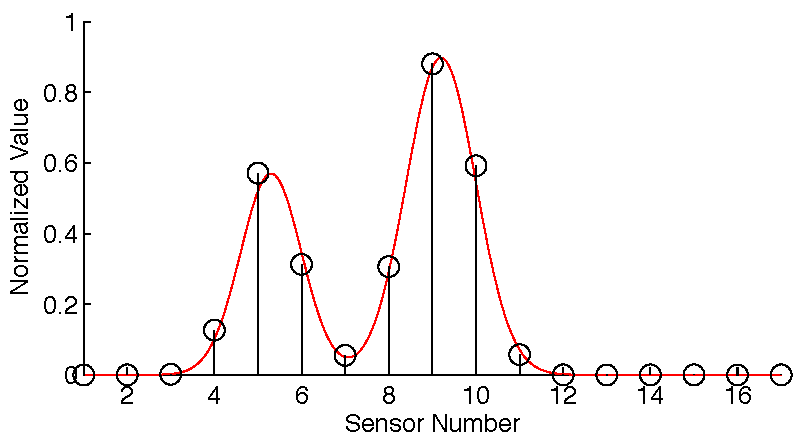
\includegraphics[width=\columnwidth]{fig1a_touch_simulation.pdf}}
\centerline{\hspace{24pt}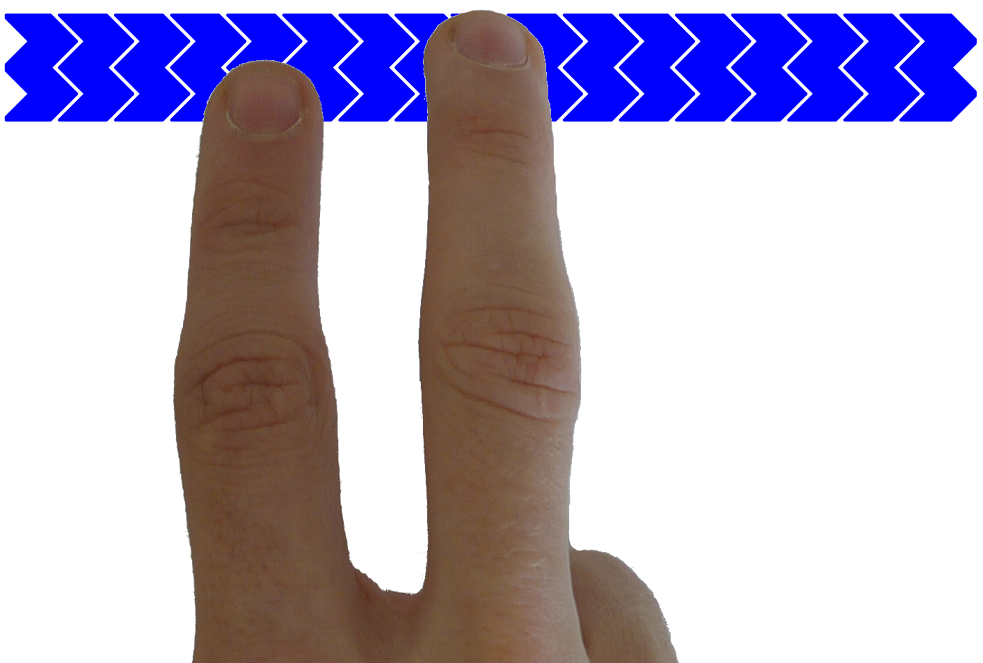
\includegraphics[width=0.8\columnwidth]{fig1b_touchkey-sharp2.png}}
%\vspace{-6pt}
\caption{Simulation of multi-centroid calculation from individual sensor readings.}
%\vspace{-12pt}
\label{McPherson:fig:slider}
\end{figure}

Though more complex to implement than resistive position sensors, capacitive sensing has the advantage of requiring no finger pressure (indeed no contact at all) to operate. With certain sensor configurations, multi-touch capability is also supported, where resistive sensors are limited to at most one or two points of contact. Capacitive sensing can be combined with existing pressure (aftertouch) keyboard systems, and unlike aftertouch, both pressed and unpressed keys can be read.

\subsection{Keyboard Sensor Design}

The TouchKeys use the PSoC 1 `CapSense' series of ICs from Cypress Semiconductor.\footnote{\url{http://www.cypress.com/products/psoc-1}} The chips contain dedicated analog hardware, including a sigma-delta ADC, to measure capacitance values on each pin. Because of this dedicated hardware, measurement time and sensor resolution significantly exceed the performance of software implementations such as the one used in the Atmel AVR (and Arduino) controllers. The Cypress chips include a microcontroller core in addition to the touch-sensing hardware; however, its performance is limited, so the TouchKeys implementation handles most data processing at a later stage.

\begin{figure}[t]
\centering
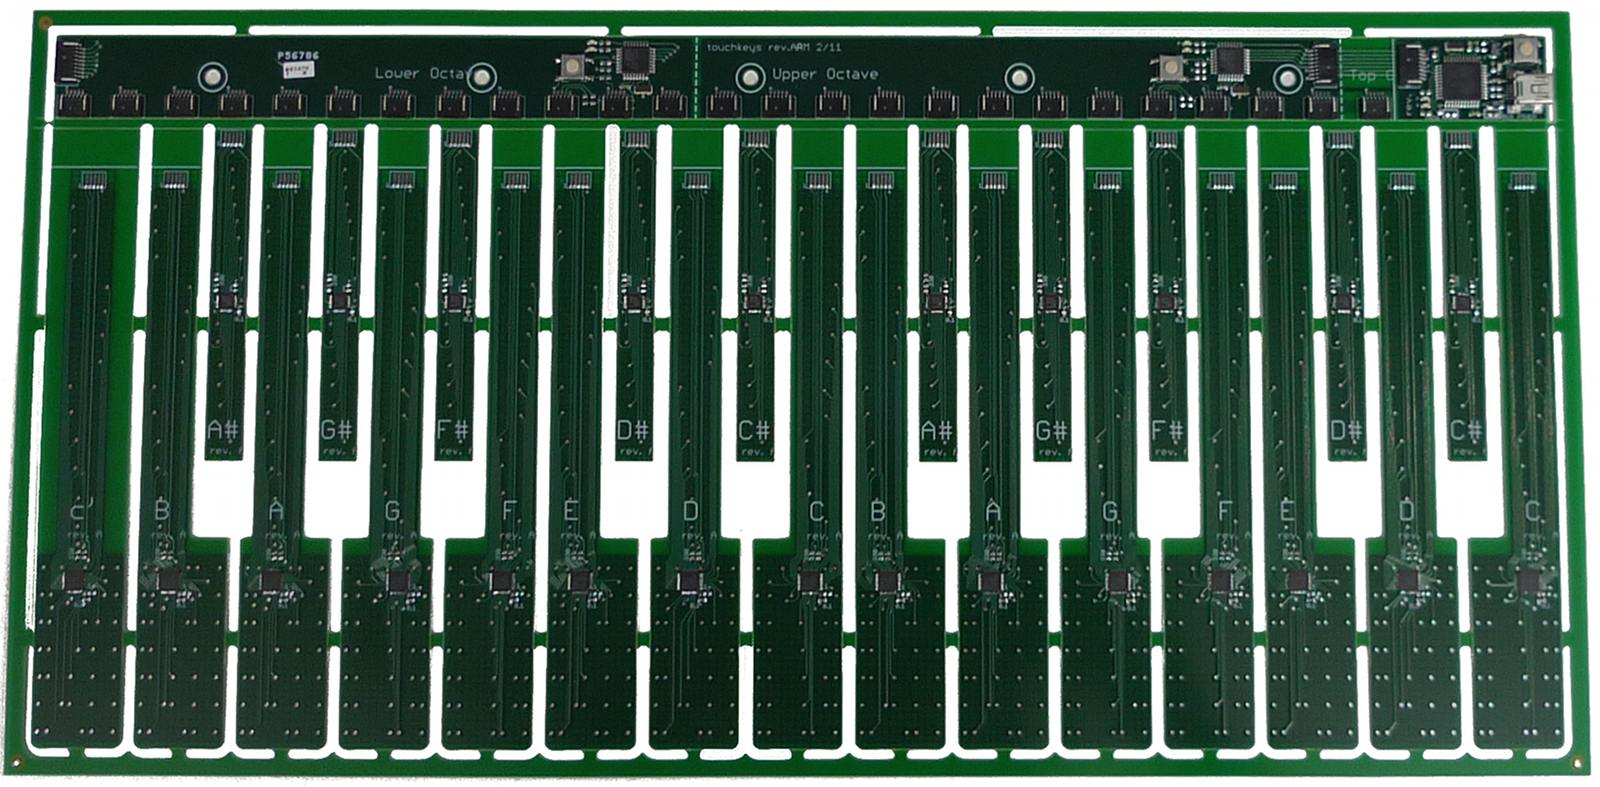
\includegraphics[width=\columnwidth]{fig2_touchkeys_bottom_small.jpg}
\caption{TouchKeys in two-octave scored panel.}
\label{McPherson:fig:board}
\end{figure}

The sensors are made from 0.8mm printed circuit boards routed to the shape of each key. Figure~\ref{McPherson:fig:board} shows a two-octave set of keys, which is fabricated as a single board with scoring that allows each key to be separated once assembled. Figure~\ref{McPherson:fig:onkeyboard} shows the keys installed on a five-octave MIDI keyboard. Plastic spacers laser-cut around the electronic components are placed underneath the circuit board to create a flat mounting surface. The sensors are attached to the keyboard with adhesive tape which creates a secure but removable bond.

\begin{figure}[t]
\centering
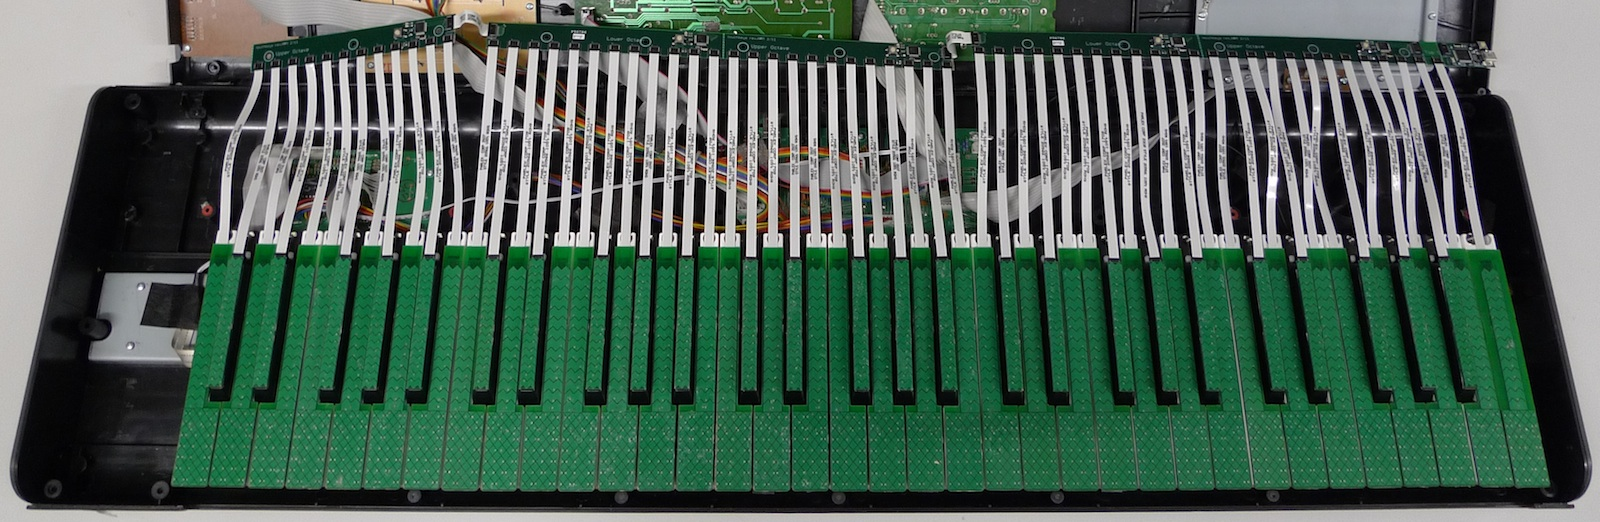
\includegraphics[width=\textwidth]{fig3_touchkeys_on_keyboard.jpg}
\caption{TouchKeys on a 61-key MIDI keyboard (open to show connections). Experiments with surface coating found the bare soldermask to produce the best feel and highest-resolution data.}
\label{McPherson:fig:onkeyboard}
\end{figure}

The black keys have 17 discrete sensor pads arranged in a single row. They are capable of sensing finger position along the lengthwise axis of the key. The white keys have 25 sensor pads, divided between a single row in the back and a grid of rows and columns in the front (Figure~\ref{McPherson:fig:layers}). The front of the white keys senses finger postion in two dimensions. Positions are calculated as the centroid of adjacent values \cite{McPherson:2011}, and up to three touches can be measured on each key.

A complete scan of 25 sensors, centroid calculations, and communication of the results via an I2C bus takes approximately 4ms. Scan rates up to 250Hz are thus possible, though because of timing constraints elsewhere in the system, 125Hz operation was found to be the most reliable. Further information on aggregation of data from multiple keys and transmission to the computer can be found in \cite{McPherson:2011}.


\subsection{PCB Design Guidelines}
Figure~\ref{McPherson:fig:layers} shows the printed circuit board layout for one key (A). The board has four layers. The top layer contains the sensor pads; the layer beneath contains traces connecting rows of pads in the two-dimensional grid; the third layer is a hatched ground plane, and the bottom layer contains the components and most signal traces. 

\begin{figure}[t]
\centering
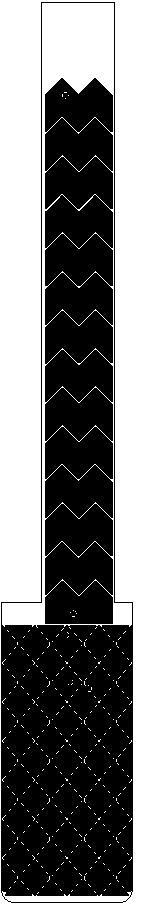
\includegraphics[width=0.18\columnwidth]{fig4a_touchkey-a_ly4.pdf}
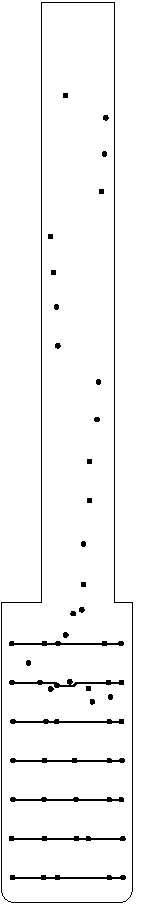
\includegraphics[width=0.18\columnwidth]{fig4b_touchkey-a_ly3.pdf}
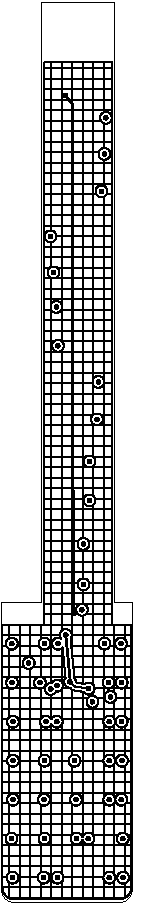
\includegraphics[width=0.18\columnwidth]{fig4c_touchkey-a_ly2.pdf}
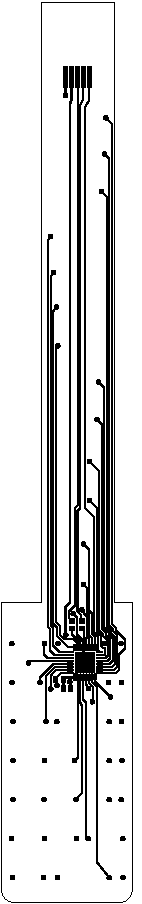
\includegraphics[width=0.18\columnwidth]{fig4d_touchkey-a_ly1.pdf}
\caption{PCB layers of one key, from top (at left) to bottom.}
\label{McPherson:fig:layers}
\end{figure}

Based on results and experiments from this design and guidance from the Cypress datasheets,\footnote{\url{http://www.cypress.com/documentation/application-notes/an65973-cy8c20xx6ahas-capsense-design-guide}} I suggest the following guidelines for capacitive touch design:

\begin{itemize}
\item{Locate the controller IC centrally. The {\it parasitic capacitance} (capacitance when no finger is present) depends on the complete conductive area, including pad and trace. Long traces should be avoided. This was a particular challenge in designing the white keys.}
\item{A ground plane is required to avoid stray interference. In a two-layer design this can be shared with components and signal traces on the bottom, but a dedicated inner layer in a four-layer design is helpful. Cypress recommends the ground plane be hatched to avoid excessive parasitic capacitance. The TouchKeys notably do not follow the recommendation that a ground plane surround the sensors on the top layer. Its absence does not seem to affect performance.}
\item{Signal traces should not cross underneath a sensor pad unless a ground plane separates the two.}
\item{Pads in an array should be V or zigzag-shaped. This ensures that a touch partially activates several adjacent pads. Similarly, pads should be close enough together that a finger activates several at once. Minimum spacing will likely be constrained by number of pins available on the controller.}
\item{Keep communication lines clear of sensor traces.}
\item{In a situation such as a physical keyboard, any action that moves the key will ideally also register as a touch location. This requires extending sensor pads as close as possible to the edges of the part.}
\end{itemize}

\subsection{Surface Coating}
The initial design of the TouchKeys \cite{McPherson:2011} used a thin plastic laminate on top of the circuit board. The intention was to more accurately simulate the look and feel of the traditional keyboard. Many types of plastic were tested, including polypropylene, PETG, Delrin, acrylic, teflon, nylon and polycarbonate. Enamel and epoxy paints were also tested. Experimentally, it was found that the laminate could be no thicker than 0.5mm on the black keys, and that on the front of the white keys, even a laminate of 0.25mm reduced performance in the two-dimensional sensor area.

Unexpectedly, many pianists indicated that the raw soldermask coating of the circuit board (an insulating layer applied during fabrication) produced a better feel than the various plastics, many of which were felt to be too sticky on the fingers. The copper sensor pads are slightly raised with respect to the etched parts of the circuit board, so the keys have a texture that was initially thought to be a drawback. However, some pianists observed that ivory keys also have a textured surface, which is not a problem in performance. The next design revision will use white and black soldermask to maintain the standard look of the keyboard.

In general, the designer can optimize any three of the following quantities at the expense of the fourth: sensor pad size, coating thickness, measurement speed and measurement resolution. The size of the TouchKey pads are constrained by the geometry of the keys, and speed and resolution were prioritized over coating thickness.

\subsection{Data Aggregation}
The controller on each key is responsible for scanning all the sensors in sequence, calculating up to three centroid locations and sizes, and transmitting this data via I2C to a second ``octave'' controller. The octave controller aggregates the data from an octave of keys and routes it to a ``host'' controller which communicates to a computer via USB \cite{McPherson:2011}. 

The host microcontroller implements a USB serial device. MIDI, even in its native USB implementation, is ill-suited for TouchKey data since controls are limited to 7 bit resolution (compared to 10 bits or more for touch position data) and Control Change messages are channel-wide rather than specific to each note. The serial data is unpacked by the computer into OSC messages which can in turn be dynamically mapped to MIDI. The mapping is discussed in the next section. The software provides a real-time visualization of key touches (Figure~\ref{McPherson:fig:visual}) which can be used in live performance or for debugging.

\begin{figure}[t]
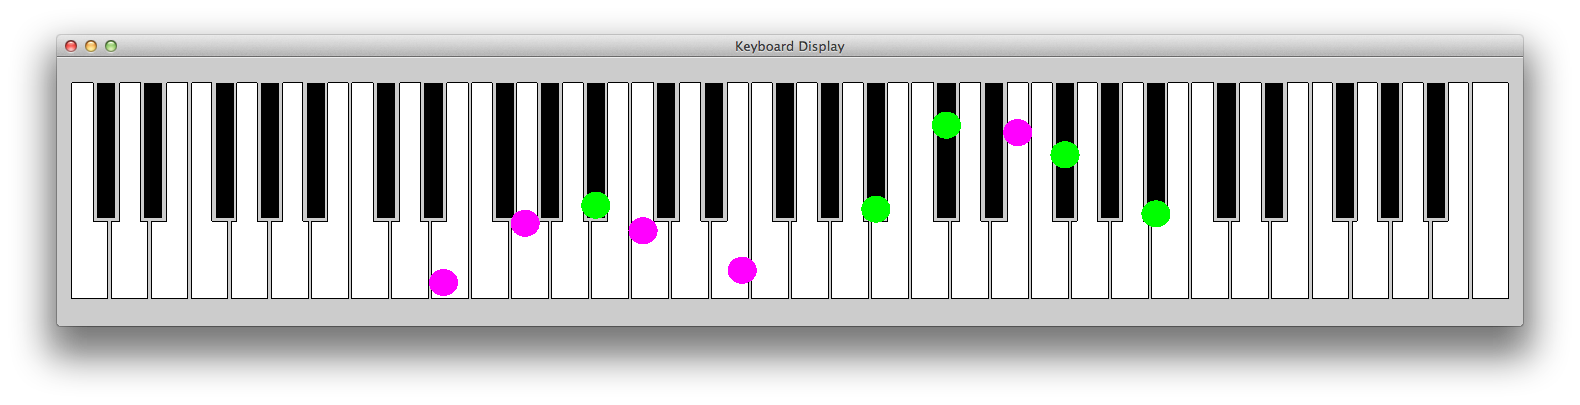
\includegraphics[width=\columnwidth]{fig5_display.png}
\caption{Real-time display of touch position.}
\label{McPherson:fig:visual}
\end{figure}

\section{Mapping Touch Data}
Open Sound Control is the native output of the TouchKey system, with messages for the following actions:
\begin{itemize}
\item{Touch onsets and releases. Distinct from MIDI note onsets and releases, this indicates when a finger touched or left the key surface.}
\item{Changes of position and contact area for each touch.}
\item{Pinch and slide gestures involving two or three fingers.}
\item{Raw data frames of all touch locations and sizes.}
\end{itemize}

The complete control system consists of touch data correlated with MIDI data from the underlying keyboard. This gives a picture of both activity on the key surfaces as well as physical key motion. Where the keyboard supports aftertouch, a form of three-dimensional sensing is available on pressed keys. All OSC messages are tagged with a MIDI note number so a synthesis program can easily correlate touch sensor and keyboard data.

\subsection{Dynamic MIDI Mapping}
Though OSC messages can be sent to any program, most commercial software synthesizers are implemented as VST or AudioUnit plugins whose parameters are set by MIDI Control Change messages. To control these plugins, a dynamic MIDI mapping system was developed (Figure~\ref{McPherson:fig:mapping}). Each touch parameter can be mapped to a different MIDI controller, to the pitch wheel, or to aftertouch. Input and output ranges are adjustable, and controls can be sent as absolute values or as relative values with respect to the original touch or note onset (see playability discussion below).

MIDI Control Change messages are limited by the fact that they apply to an entire channel, prohibiting polyphonic control. The mapping engine allocates a new MIDI channel for each Note On message, rebroadcasting it to one of several identical copies of a synth plugin, each listening on a different channel. Before the Note On is sent, Control Change messages are sent on the same channel based on the current touch information, ensuring that the controls take their proper position before the note begins. If a Note On arrives before any frames of touch data for the same key, retransmission is delayed for up to 10ms to allow touch data to come in. In practice, this is only necessary for the fastest strikes originating above the keyboard.

\begin{figure}[t]
\centering
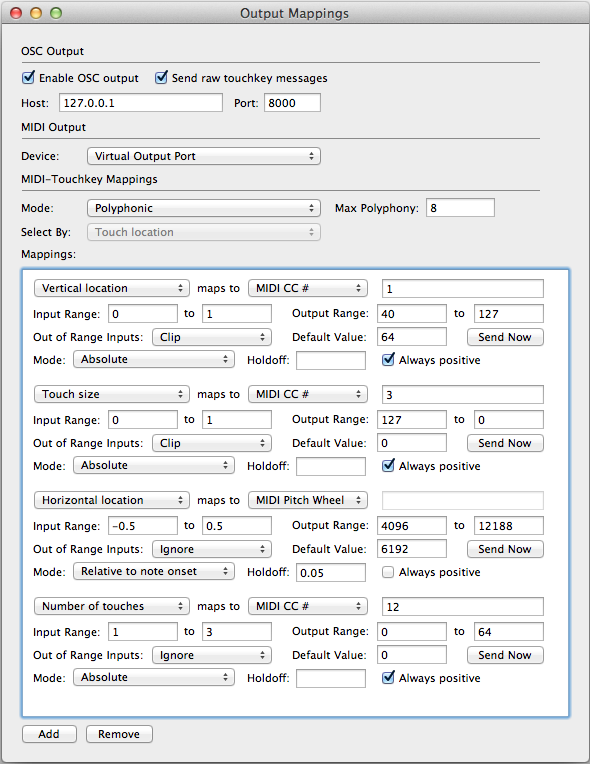
\includegraphics[width=0.85\columnwidth]{fig6_mappings2.png}
\caption{Mapping editor assigns parameters to multi-channel MIDI messages.}
\label{McPherson:fig:mapping}
\end{figure}

\subsection{Control and Playability}

On the piano, the location of each touch is partially constrained by fingering. Mappings based on the absolute position of each finger in each dimension will thus be challenging. Composer John Eaton remarked of the Moog touch-keyboard: ``It's very difficult to play. But an instrument should be difficult to play. That's the only way to master musical materials, by overcoming these difficulties'' \cite{Star-Ledger:2006}. 

Certain simple strategies can produce a more easily-learned instrument, including tracking deviation from initial touch position (motions which rarely occur in traditional technique) or mapping to parameters which are expressive but which do not require precise control to produce acceptable results (e.g. pluck position on a virtual string model). Detailed user evaluation of mappings is currently underway; preliminary results indicate that the two principles above produce usable results.

\subsection{Example: Analog-Modeling Synth}
The TouchKeys were configured to control the FXpansion Strobe\footnote{\url{https://www.fxpansion.com/products/dcamsynthsquad/}} analog-modeling monosynth. Eight copies of the synth were hosted in Apple's AULab environment. Each copy was configured identically but on a different MIDI channel. The TouchKey mapping engine dynamically routed notes from the host keyboard to one copy of the synth, and the touch mappings in Figure~\ref{McPherson:fig:mapping} were used to send Control Change messages to specific channels:
\begin{itemize}
\item{Vertical (front-back) position controlled the cutoff of a low-pass resonant filter.}
\item{Horizontal position controlled the pitch wheel to bend notes up or down. This feature is presently only available on the white keys since they sense touch on two axes; it allows an intuitive ``vibrato'' motion (rocking finger on the key).}
\item{Contact area was mapped to the level of white noise mixed into the main oscillator output. Normal technique (large contact area) creates a pure sawtooth tone, but special effects can be generated by playing on the very tip of the finger or the fingernail. When this is coupled with sharp attack and long release time, interesting percussive sounds can result.}
\item{Number of fingers (1-3) was mapped the number of stacked oscillators, each of which was slightly detuned so that multiple touches produced a wider sound.}
\end{itemize}

This is only one of many possible mappings, but it demonstrates how the TouchKeys can be configured to operate with standard VST/AudioUnit plug-ins.

\section{Conclusion}
This paper has presented the TouchKeys, a multi-touch augmentation of the traditional keyboard. The sensor system can be installed atop acoustic or electronic keyboards, where it provides continuous multidimensional control over each note while retaining the tactile feedback that is important to keyboard performance.

An important area of future exploration is the connection of the TouchKeys to the magnetic resonator piano (MRP), an electromagnetically-augmented acoustic piano developed by the author \cite{McPherson:2010}. Electromagnets inside the acoustic piano can shape the amplitude, frequency and timbre of each note in real time, expanding the piano's musical vocabulary. Multidimensional keyboard control is a natural extension of this project, and indeed, performers frequently suggest finger motion along the keys as a means of note-shaping.

\section*{Author Commentary: Taking an Augmented Keyboard from the Lab to the Stage}
\paragraph{Andrew McPherson}

While the basic layout of the keyboard has changed little in over 500 years, generations of inventors have attempted to circumvent a basic limitation of most keyboard instruments: that the keyboard is essentially discrete. The performer can control the onset and release of each note but has comparatively few ways to shape what happens in the middle. From Leonardo da Vinci's 15th-century sketches of the \lq viola organista \rq to 18th-century keyboard variants of Benjamin Franklin's glass harmonica to Hugh Le Caine's 1948 Electronic Sackbut, luthiers have used the technology of their day to pursue something of an instrumental holy grail: an instrument combining the flexibility of the keyboard with the continuous note shaping of the violin or voice \cite{McPherson:2015a}.

The role of the keyboard within the NIME community is complex. On one hand, many augmented keyboards and keyboard-inspired interfaces have appeared at NIME. On the other hand, the keyboard might also be seen as a mental obstacle to be overcome on the way to new forms of musical interaction. Indeed, the subtitle of Miranda and Wanderley's comprehensive 2006 text on digital musical instruments is ``Control and Interaction Beyond the Keyboard'' \cite{Miranda:2006}.

TouchKeys follows in a long line of new keyboard technology, most notably Robert Moog's Multiply-Touch-Sensitive keyboard \cite{Moog:1990}. In my view, its most important lesson for the NIME community is to highlight the power and musical potential of performer familiarity. For novel instruments, the performer's experience level quickly becomes the dominant limitation, since few musicians are able or willing to devote years of practice to become proficient on an unfamiliar instrument.

In its basic physical layout and in its particular mapping strategies, TouchKeys builds on existing keyboard skills, letting pianists control new effects while minimally interfering with traditional playing techniques. It can be seen as a manifestation of Tremblay and Schwartz's principle of \lq recycling virtuosity\rq \cite{Tremblay:2010} or of Perry Cook's recommendation on \lq leveraging expert technique\rq \cite{Cook:2001}.

Partly because of the close connection to existing piano technique, TouchKeys has gone on to be used by quite a few musicians. In 2013, after 5 generations of hardware design, I ran a Kickstarter campaign which shipped self-install kits and prebuilt instruments to musicians in 20 countries. Since then, I've built and shipped another large production run, and the project is now in the process of spinning out of the university into an independent startup company. It has been enjoyable, and also a learning experience, to build a community of performers and composers around this instrument.

A limitation inherent to the TouchKeys design is that it is a controller, generating MIDI or OSC messages to manipulate external sounds. Compared to my other augmented keyboard project, the magnetic resonator piano \cite{McPherson:2015a}, the lack of an identifiable \lq TouchKeys\rq sound has meant that it less easily generates a signature identity for new compositions. Of course, this is balanced by the flexibility that it gives performers to integrate it into their own workflow. 

There remains a question about whether a generic separation between controller and sound generator will ever achieve the level of control intimacy provided by fully integrated systems (whether acoustic or electronic). Of course, even for re-mappable controllers, the performer can decide to settle on just one configuration and learn it over many years. However, there may be a temptation to regularly change settings, in which case the performer's relationship with the instrument may relate more to its breadth of possibilities than the depth and subtlety of any one configuration. A related question is whether the designer, in seeking to make a controller generically applicable, will forego certain idiosyncrasies of behaviour that could be exploited in a fully integrated instrument.

One general challenge I have found, which is not uncommon in NIME, is navigating the tension between academic and commercial/musical expectations. Most academic fields prioritise novelty over continuing development; the pressure is to develop a project sufficiently to publish a high-quality paper, then leave it aside in favour of the next research project. But creating a digital musical instrument suitable for the highest echelons of performance can take many rounds of development, user testing and refinement, and not all of these technical details are publishable. Instead, the most interesting research outcomes are the things we can learn about the players themselves and the way they engage with technology. In my opinion, the human aspect of NIME is an area where many broad and fascinating questions remain to be explored.

\section*{Expert Commentary: Turning the Piano Keyboard Inside Out}
\paragraph{Palle Dahlstedt}

Many musicians have tried to extend control over piano tone beyond that initial attack. Electronics have been used for sound processing, sensors have been added, and pianists have reached inside the instrument to interact directly with the strings. But in my title, I refer not to Sarah Nicolls' Inside out piano \cite{Nicolls:2010}, but to what Andrew McPherson did conceptually to the piano keyboard with the introduction of his TouchKeys sensor system \cite{McPherson:2012a}.

There is a kind of inverse correlation between polyphony of sound and intimacy of control in musical instruments, distributing the cognitive load of the player over available variables. In one end of the scale is the human voice, with supreme control over monophonic sound. Somewhere in the middle is the violin with intimate continuous control and some polyphonic capabilities, but in polyphonic playing individual control is reduced. Near the other end, just before the church organ, is the piano, where tonal control stops when the hammer leaves the string, but this is compensated by structural complexity and focus on relationship (in time and dynamics) between simultaneous and succeeding notes.

With TouchKeys, McPherson has turned the piano keyboard inside out, and effectively transformed it from one end of the scale to the other, at least on the interface side. High-resolution multitouch sensing on each key turns the focus of the pianist from structure and multiplicity in pitch and time, to the potential of intimate gestural micro-narratives, and high-dimensional control of single sounds. The mental charts have to be redrawn, and as a pianist, my attention lands carefully on the key surface to explore this potential. The rest of the keyboard is still there in the background, blurred and distant.

McPherson is an instrument maker, a toolmaker, in the classic sense: a virtuoso engineer and craftsman, economical and rational, who constructs an extension of an existing interface in close collaboration with musicians, and makes it available to them. McPherson's respect for musicians is evident, e.g, in his detailed discussion about the key surface material---he is aware that minute differences in texture and friction affect playability and musicianship. So he asks the players.

Further research and experimentation is needed---since TouchKeys is an open-ended interface, and as such it is but one of three main components of an instrument, followed by the mapping and the sound engine. To design mappings that fully (whatever that means) utilize the gestural possibilities in a musically meaningful way is highly nontrivial, and different solutions will be musically meaningful in very different ways. McPherson only touches upon mapping issues in his text, just making sure that core gestural data is available. I think this is a good decision. It makes his invention more open, and allows for diverse approaches and continued research.

In comparison to related interfaces, such as the Haaken Continuum \cite{Haken:1998}, TouchKeys allows the pianist to dive into the single key (or single note)---instead of expanding the whole keyboard into a large continuum. It keeps the keyboard paradigm, but expands it inwards. This means a lot for playability. It makes it accessible for keyboard players, easy to conceptualize with regards to synthesis and processing, and does not get in the way of hard-earned playing skills---but augments them instead.

In a normal multi-touch surface, e.g., a tablet computer, each finger generates a blob, with location (and possibly area). The identity of the blob has to be inferred from initial coordinates or a similar mechanism. With TouchKeys you instead have a large set of separate multitouch surfaces (albeit small), each with continuous properties. This reminds me more of David Wessel's last performance instrument \cite{Wessel:2007}, based around an array of small touch surfaces, allowing for intimate complex x/y/z gestures with distinct identities.

As a pianist and keyboard improviser, I see many possibilities for musical applications. The most obvious (and boring) is to add continued control of a sounding note (pitch, dynamics, timbre), through relative movement of the finger. The ability to sense touch on unpressed keys could be used for control of formant resonances and filtering---or spectral muting---where pressed keys generate the carrier sound. Touch gestures on keys (pressed or unpressed) allows for bowing, scratching or tapping metaphors to inject energy into physical synthesis models. In my own approaches to augmented piano \cite{Dahlstedt:2015}, I have tried to transcend the zeroeth-order mapping paradigm using dynamic mappings and virtual string models. In the next iteration, TouchKeys will play an important role. The possibilities are endless, and will keep us busy.

In a non-invasive way, keeping the main structure of the original interface, TouchKeys adds so many degrees of freedom that it has the potential to completely transform keyboard playing. It is no longer only about discrete entities---inside those, McPherson have opened an expressive continuum, effectively turning the keyboard inside out. And I'm going in.

